One of the hardest part of creating and training \gls{ml} models is accurately evaluating their performance. How can you known if your model is giving out accurate predictions ? What is accuracy, and how can we precisely define it ? Understanding the type of errors a detection network can make is a crucial part in enhancing their performance in real world situation. In this section, we will present metrics used in detection and classification tasks.


\section{Type of Errors}
In a classification task, where a model is ask to classify an item into a fixed number of categories based on input characteristics. A model will predict the class of a given item, for example if an input image contains a cat or a dog. In doing so, the model can make mistakes. When predicting a particular class, there are 2 type of predictions that can be made: positive or negative, and those predictions can be true or false. When a network correctly predicts that an image contains a cat, it is a true positive. When it predicts that there is no dog when there is one, this is a false negative.

All in all, there are 4 categories of predictions: True Positive (TP), False Positive (FP), True Negative (TN) and False Negative (TN). 
\section{Precision and Recall}
Precision is defined as "the fraction of detections reported by model that were correct" and recall is "the fraction of detections reported by the model which were correct"\cite[p.411]{Goodfellow2016}. We can see those concepts visualised in Figure~\ref{fig:precRecall}. In that Figure, the precision would be equal to the number True Positives in green divided by number of selected elements \textit{i.e.} the green and red sets combined. The recall would be equal to the number of true positives over the total number of relevant elements or the dark gray set and the green set combined. 

\begin{figure}[h]
  \centering
  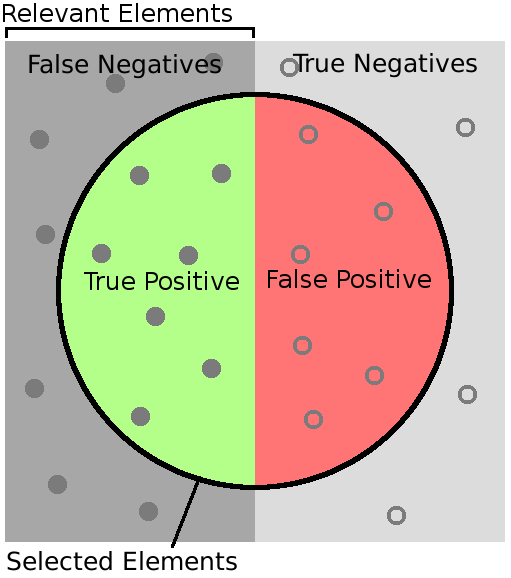
\includegraphics[width=0.7\textwidth]{precisionRecall}
	\caption[]{Precision and recall on a classification task.}
  \label{fig:precRecall}
\end{figure}

Precision and recall allows us to quantify with more accuracy the quality of a model than just the number of errors that it makes. For example, in the case of a model trying to detect a rare event like a disease that would infect only a small fraction of the population, say one in a million, \textbf{a detector that would always infer that a person is not sick would be able to attain a $99.9999\%$ accuracy.} However, while this detector would achieve a very high precision, it would have a very bad recall, which would indicate that it is not a very good model after all.

\section{Intersection over Union (IoU)}\label{iouExplanation}
The intersection over union, or Jaccard Index quantifies the accuracy of the bounding box prediction. \gls{iou} measure the quality of a bounding box : if the predicted bounding box overlaps significantly with the ground truth bounding box, then it should have a low score, and inversely if the prediction does not overlap with the ground truth. The \gls{iou} is given by the following equation:

\begin{equation}
	IoU = \frac{\text{area}(BBox_{truth} \cap BBox_{pred})} {\text{area}(BBox_{truth} \cup BBox_{pred})}
\end{equation}

\begin{figure}
  \centering
  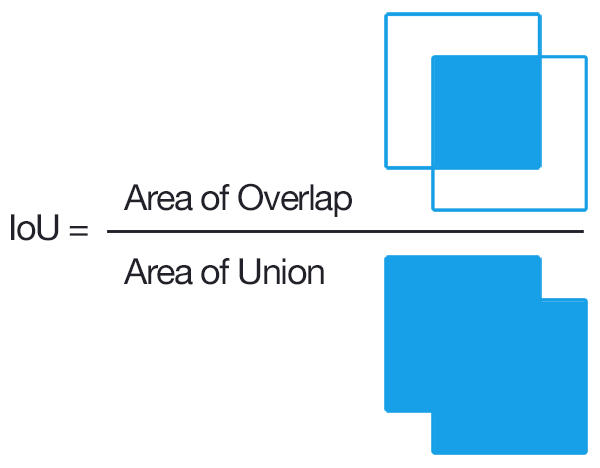
\includegraphics[width=0.5\textwidth]{iou}
	\caption[Intersection over Union]{Intersection over Union\\\textbf{Source}: https://www.pyimagesearch.com/2016/11/07/intersection-over-union-iou-for-object-detection/}
  \label{fig:iou}
\end{figure}

Generally a detection is considered correct if the $\text{IoU} \geq 0.5$; this threshold is also used when computing the \gls{map}. It should also be noted that the \gls{iou} is not the only way to measure how good a bounding box is. Improvements on this metric has been done that gives out a better measure on the quality of the box, such as the \gls{giou}\cite{giou}, \gls{diou}\cite{diou} and \gls{ciou}\cite{diou}. Those metrics are used in our model, and are presented in Section~\ref{ious}. 

\section{Mean Average Precision (mAP) and F1-Score}
The F1-Score is a measure of test accuracy. It is the harmonic mean of precision and recall :
\begin{equation}
	2 \cdot \frac{precision \cdot recall}{precision + recall}
\end{equation}

The mean average precision is the metric used by the COCO dataset\cite{msCOCO}. As said above, when the IoU between the prediction and the ground truth is over 0.5, the prediction is considered a valid detection. 

\section{Evaluating a model}
Computing those metrics and analyzing them allows a researcher to better understand the behavior of its model, and preventing degenerate behavior. It should however be noted that those metrics do not always give out accurate or useful information. In that case, only knowledge and experience of the usual issues can help.

For example, it can happen that a model will always infer one class other another, for any kind of object and still outputs good accuracy \footnote{This often happens in the case of an unbalanced dataset, where one class appear more often than any other.}. It can also be the case that a metric is very sensible at a some scale of errors but not at others: the L2 distance for example grows quadratically and outputs small distances when the L1 distance is below 1, but very high values that might be hard to optimize for when the L1 distance is over 1.

The only way to diagnose those issues will be to manually inspect the prediction of the model, and carefully choosing the metrics used. 

